\documentclass[a4paper,12pt]{article}
\usepackage[utf8]{inputenc}
\usepackage[T1]{fontenc}
\usepackage[portuguese]{babel}
\usepackage{geometry}
\geometry{margin=2.5cm}
\usepackage{graphicx}
\usepackage{hyperref}
\usepackage{titlesec}
\usepackage{enumitem}
\usepackage{listings}
\usepackage{xcolor}
\usepackage{booktabs}
\usepackage{array}
\usepackage{mathptmx}
\usepackage{appendix}
\usepackage{caption}

\usepackage{tikz}
\usetikzlibrary{shapes.geometric, arrows.meta, positioning, calc}

% Configuração do estilo de código Python
\lstdefinestyle{python}{
    language=Python,
    basicstyle=\ttfamily\small,
    keywordstyle=\color{blue!70!black}\bfseries,
    stringstyle=\color{orange!80!black},
    commentstyle=\color{gray}\itshape,
    numberstyle=\tiny\color{gray},
    numbers=left,
    stepnumber=1,
    numbersep=8pt,
    backgroundcolor=\color{gray!8},
    frame=single,
    rulecolor=\color{gray!40},
    breaklines=true,
    breakatwhitespace=true,
    showstringspaces=false,
    tabsize=4,
    captionpos=b
}

\hypersetup{
    colorlinks=true,
    linkcolor=blue!60!black,
    urlcolor=blue!60!black
}

\title{\textbf{Estudo de arquiteturas de CNN no dataset \textit{CIFAR-10}}}
\author{Gabriel Brum}
\date{\today}

\begin{document}

\maketitle
\tableofcontents
\newpage

% ===========================================================================
\section{Introdução}
% ===========================================================================

Esta seção expõe as topologias escolhidas, os hiperparâmetros selecionados e suas respectivas justificativas.

O código foi desenvolvido em Python, executado no servidor do grupo de pesquisa LIPAI, e está disponível no \textit{github} [\url{}].


\subsection{CNN-A: A menor arquitetura}

\begin{lstlisting}[style=python, caption={Arquitetura A (CNN simples).}]
"CNN_A": {
        "conv_configs": [
            {"filters": 32, "kernel": 3},   # conv1: 32 filtros 3x3
            {"filters": 64, "kernel": 3},   # conv2: 64 filtros 3x3
        ],
        "fc_sizes"   : [256, 128],
        "dropout_p"  : 0.0,
        "optimizer"  : "adam",
        "lr"         : 1e-3,
    }
\end{lstlisting}

Esta arquitetura visa ser a \textit{baseline}, onde não realizamos regularização, assim espera-se que haja \textit{overfitting} e que a acurácia de validação seja inferior às demais arquiteturas.
Em \textit{Listing 1}, está o código da arquitetura CNN-A, que consiste em duas camadas convolucionais seguidas por duas camadas totalmente conectadas (fully connected). As camadas convolucionais utilizam filtros de 3x3, com 32 e 64 filtros respectivamente, e são seguidas por camadas de pooling para reduzir a dimensionalidade. As camadas totalmente conectadas possuem 256 e 128 neurônios, respectivamente, e não utilizam dropout para regularização. O otimizador escolhido é o Adam, com uma taxa de aprendizado de 0.001.
Para melhor visualização, o esquema presente na Figura 1 mostra o fluxo entre as camadas.

\begin{figure}[htpb]
    \centering
    \begin{tikzpicture}[
        % 1. DEFINIÇÃO DOS ESTILOS VISUAIS
        base/.style={
            draw, align=center, minimum height=1.2cm, minimum width=5.5cm, 
            font=\sffamily, rounded corners, thick
        },
        % Blocos Convolucionais (fundo azul claro, borda azul escura)
        conv/.style={base, fill=blue!10, draw=blue!80},
        % Blocos Fully Connected (fundo roxo claro, borda roxa escura)
        fc/.style={base, fill=purple!10, draw=purple!80},
        % Blocos de Entrada/Saída/Achatamento (fundo cinza)
        io/.style={base, fill=gray!10, draw=gray!70, minimum height=0.8cm},
        % Estilo das setas
        arrow/.style={thick, ->, >=stealth}
    ]

        % 2. DEFINIÇÃO DOS BLOCOS (NÓS)
        \node[io] (in) {Entrada RGB \\ (32x32x3)};
        
        % O 'below=0.5cm of in' posiciona este bloco automaticamente abaixo da entrada
        \node[conv, below=0.5cm of in] (c1) {Conv1: 32 filtros (3x3) + ReLU \\ MaxPool (2x2) \\ Saída: 16x16x32};
        
        \node[conv, below=0.5cm of c1] (c2) {Conv2: 64 filtros (3x3) + ReLU \\ MaxPool (2x2) \\ Saída: 8x8x64};
        
        \node[io, below=0.5cm of c2] (flat) {Flatten \\ (Vetor de 4096 características)};
        
        \node[fc, below=0.5cm of flat] (fc1) {FC1: 256 neurônios + ReLU \\ (Sem Dropout)};
        
        \node[fc, below=0.5cm of fc1] (fc2) {FC2: 128 neurônios + ReLU \\ (Sem Dropout)};
        
        \node[io, below=0.5cm of fc2] (out) {Camada de Saída: 10 classes};

        % 3. LIGAÇÃO DAS SETAS
        \draw[arrow] (in) -- (c1);
        \draw[arrow] (c1) -- (c2);
        \draw[arrow] (c2) -- (flat);
        \draw[arrow] (flat) -- (fc1);
        \draw[arrow] (fc1) -- (fc2);
        \draw[arrow] (fc2) -- (out);

    \end{tikzpicture}
    
    \caption{Arquitetura CNN-A: Baseline Simples (Otimizador: Adam, LR: 1e-3, Dropout: 0.0)}
    \label{fig:cnn_a}
\end{figure}

\subsection{CNN-B: A arquitetura média}

\begin{lstlisting}[style=python, caption={Arquitetura B (CNN média).}]
"CNN_B": {
        "conv_configs": [
            {"filters": 64,  "kernel": 5},  # conv1: 64 filtros 5x5
            {"filters": 128, "kernel": 3},  # conv2: 128 filtros 3x3
            {"filters": 128, "kernel": 3},  # conv3: 128 filtros 3x3
        ],
        "fc_sizes"   : [200, 200],
        "dropout_p"  : 0.1,
        "optimizer"  : "adam",
        "lr"         : 1e-3,
    }
\end{lstlisting}

A arquitetura CNN-B é uma versão intermediária, com mais camadas e regularização leve. Como exposto em \textit{Listing 2} ela possui três camadas convolucionais, com 64 filtros de 5x5 na primeira camada e 128 filtros de 3x3 nas duas camadas seguintes. As camadas totalmente conectadas têm 200 neurônios cada, e um dropout de 0.1 é aplicado para reduzir o risco de overfitting. O otimizador e a taxa de aprendizado são os mesmos da CNN-A.
A Figura 2 ilustra a estrutura da CNN-B, destacando as diferenças em relação à CNN-A, como o aumento no número de camadas e a introdução do dropout.

\begin{figure}[htpb]
    \centering
    \begin{tikzpicture}[
        base/.style={
            draw, align=center, minimum height=1.2cm, minimum width=5.5cm, 
            font=\sffamily, rounded corners, thick
        },
        conv/.style={base, fill=blue!10, draw=blue!80},
        fc/.style={base, fill=purple!10, draw=purple!80},
        io/.style={base, fill=gray!10, draw=gray!70, minimum height=0.8cm},
        arrow/.style={thick, ->, >=stealth}
    ]

        % Nós (Blocos)
        \node[io] (in) {Entrada RGB \\ (32x32x3)};
        
        \node[conv, below=0.5cm of in] (c1) {Conv1: 64 filtros (5x5) + ReLU \\ MaxPool (2x2) \\ Saída: 16x16x64};
        
        \node[conv, below=0.5cm of c1] (c2) {Conv2: 128 filtros (3x3) + ReLU \\ MaxPool (2x2) \\ Saída: 8x8x128};
        
        \node[conv, below=0.5cm of c2] (c3) {Conv3: 128 filtros (3x3) + ReLU \\ MaxPool (2x2) \\ Saída: 4x4x128};
        
        \node[io, below=0.5cm of c3] (flat) {Flatten \\ (Vetor de 2048 características)};
        
        \node[fc, below=0.5cm of flat] (fc1) {FC1: 200 neurônios + ReLU \\ Dropout (0.1)};
        
        \node[fc, below=0.5cm of fc1] (fc2) {FC2: 200 neurônios + ReLU \\ Dropout (0.1)};
        
        \node[io, below=0.5cm of fc2] (out) {Camada de Saída: 10 classes};

        % Setas
        \draw[arrow] (in) -- (c1);
        \draw[arrow] (c1) -- (c2);
        \draw[arrow] (c2) -- (c3);
        \draw[arrow] (c3) -- (flat);
        \draw[arrow] (flat) -- (fc1);
        \draw[arrow] (fc1) -- (fc2);
        \draw[arrow] (fc2) -- (out);

    \end{tikzpicture}
    \caption{Arquitetura CNN-B: Média (Otimizador: Adam, LR: 1e-3, Dropout: 0.1)}
    \label{fig:cnn_b}
\end{figure}

\subsection{CNN-C: A arquitetura grande}

\begin{lstlisting}[style=python, caption={Arquitetura C (CNN grande).}]
"CNN_C": {
        "conv_configs": [
            {"filters": 32,  "kernel": 3},
            {"filters": 64,  "kernel": 3},
            {"filters": 128, "kernel": 3},
            {"filters": 128, "kernel": 3},
        ],
        "fc_sizes"   : [256, 128],
        "dropout_p"  : 0.3,
        "optimizer"  : "sgd",
        "lr"         : 1e-2,   
    }
\end{lstlisting}

Aqui a arquitetura é mais robusta, com quatro camadas convolucionais e uma regularização mais forte. Conforme mostrado em \textit{Listing 3}, as camadas convolucionais têm 32, 64, 128 e 128 filtros de 3x3, respectivamente. As camadas totalmente conectadas possuem 256 e 128 neurônios, com um dropout de 0.3 para combater o overfitting. O otimizador escolhido é o SGD, que geralmente requer uma taxa de aprendizado maior (1e-2) em comparação ao Adam.
A Figura 3 apresenta a estrutura da CNN-C, evidenciando o aumento no número de camadas e a mudança no otimizador, que pode impactar significativamente o processo de treinamento e a convergência do modelo.

\begin{figure}[htpb]
    \centering
    \begin{tikzpicture}[
        base/.style={
            draw, align=center, minimum height=1.2cm, minimum width=5.5cm, 
            font=\sffamily, rounded corners, thick
        },
        conv/.style={base, fill=blue!10, draw=blue!80},
        fc/.style={base, fill=purple!10, draw=purple!80},
        io/.style={base, fill=gray!10, draw=gray!70, minimum height=0.8cm},
        arrow/.style={thick, ->, >=stealth}
    ]

        % Nós (Blocos)
        \node[io] (in) {Entrada RGB \\ (32x32x3)};
        
        \node[conv, below=0.5cm of in] (c1) {Conv1: 32 filtros (3x3) + ReLU \\ MaxPool (2x2) \\ Saída: 16x16x32};
        
        \node[conv, below=0.5cm of c1] (c2) {Conv2: 64 filtros (3x3) + ReLU \\ MaxPool (2x2) \\ Saída: 8x8x64};
        
        \node[conv, below=0.5cm of c2] (c3) {Conv3: 128 filtros (3x3) + ReLU \\ MaxPool (2x2) \\ Saída: 4x4x128};
        
        \node[conv, below=0.5cm of c3] (c4) {Conv4: 128 filtros (3x3) + ReLU \\ MaxPool (2x2) \\ Saída: 2x2x128};
        
        \node[io, below=0.5cm of c4] (flat) {Flatten \\ (Vetor de 512 características)};
        
        \node[fc, below=0.5cm of flat] (fc1) {FC1: 256 neurônios + ReLU \\ Dropout (0.3)};
        
        \node[fc, below=0.5cm of fc1] (fc2) {FC2: 128 neurônios + ReLU \\ Dropout (0.3)};
        
        \node[io, below=0.5cm of fc2] (out) {Camada de Saída: 10 classes};

        % Setas
        \draw[arrow] (in) -- (c1);
        \draw[arrow] (c1) -- (c2);
        \draw[arrow] (c2) -- (c3);
        \draw[arrow] (c3) -- (c4);
        \draw[arrow] (c4) -- (flat);
        \draw[arrow] (flat) -- (fc1);
        \draw[arrow] (fc1) -- (fc2);
        \draw[arrow] (fc2) -- (out);

    \end{tikzpicture}
    \caption{Arquitetura CNN-C: Profunda (Otimizador: SGD, LR: 1e-2, Dropout: 0.3)}
    \label{fig:cnn_c}
\end{figure}
% ===========================================================================
\section{Resultados}
% ===========================================================================

\subsection{CNN-A}

\subsubsection{Acurácia, Loss e Predições}
A arquitetura CNN-A atingiu uma acurácia de teste de 77.38\%. O critério de parada antecipada (\textit{early stopping}) foi acionado na época 25, indicando que o modelo começou a saturar e perder capacidade de generalização precocemente. Apesar da ausência de camadas de \textit{dropout}, a aplicação do \textit{Data Augmentation} no pré-processamento das imagens mitigou o sobreajuste severo. A Figura \ref{fig:cnn_a_hist} ilustra o histórico de treinamento, onde a função de custo (\textit{loss}) de validação estabiliza na faixa de 0.69, não acompanhando a queda contínua da perda de treinamento. A Figura \ref{fig:cnn_a_pred} apresenta uma amostra das predições realizadas no conjunto de teste.

\begin{figure}[htpb]
    \centering
    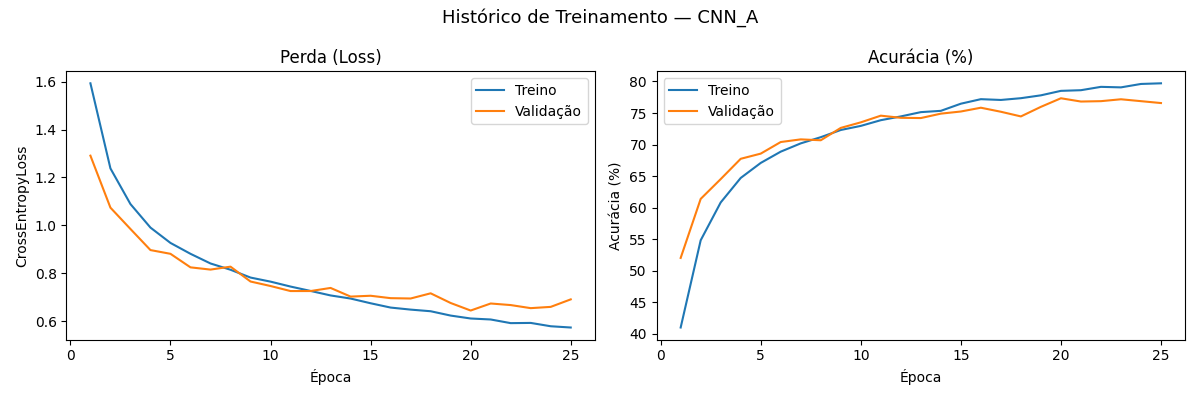
\includegraphics[width=0.9\textwidth]{output/CNN_A_historico.png}
    \caption{Histórico de \textit{Loss} e Acurácia para a CNN-A.}
    \label{fig:cnn_a_hist}
\end{figure}

\begin{figure}[htpb]
    \centering
    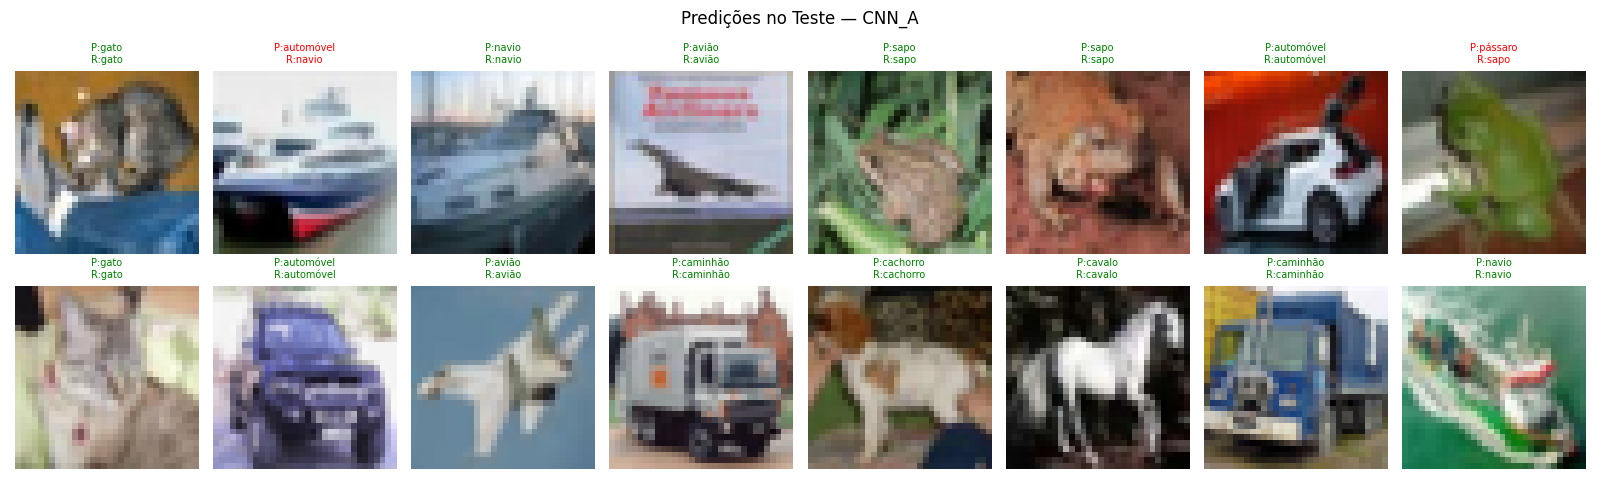
\includegraphics[width=0.8\textwidth]{output/CNN_A_predicoes.png}
    \caption{Amostra de predições da arquitetura CNN-A no conjunto de teste.}
    \label{fig:cnn_a_pred}
\end{figure}

\subsubsection{Filtros e \textit{Feature Maps}}
A análise da primeira camada convolucional (Figura \ref{fig:cnn_a_filtros}) revela que os filtros $3 \times 3$ aprenderam a detectar padrões de baixo nível espacial, consistindo principalmente em detectores de bordas simples e transições abruptas de cor. Os mapas de ativação (Figura \ref{fig:cnn_a_mapas}), extraídos da última camada convolucional, evidenciam a captação das silhuetas dos objetos, porém com características topológicas primárias, compatíveis com a menor profundidade da rede.

\begin{figure}[htpb]
    \centering
    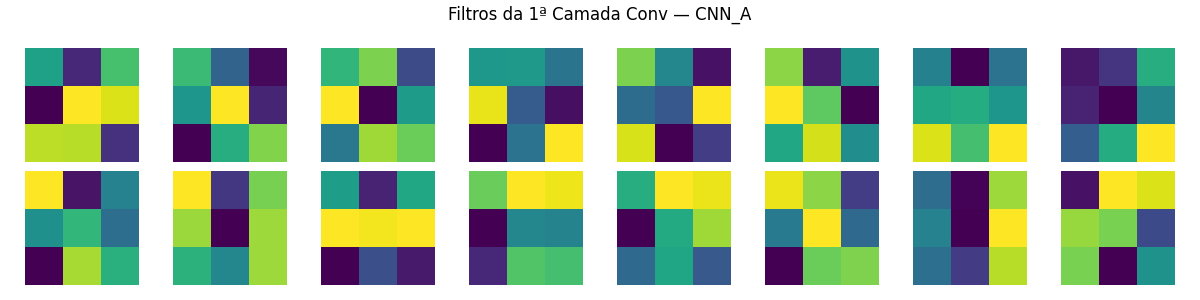
\includegraphics[width=0.7\textwidth]{output/CNN_A_filtros.png}
    \caption{Filtros aprendidos na primeira camada convolucional da CNN-A.}
    \label{fig:cnn_a_filtros}
\end{figure}

\begin{figure}[htpb]
    \centering
    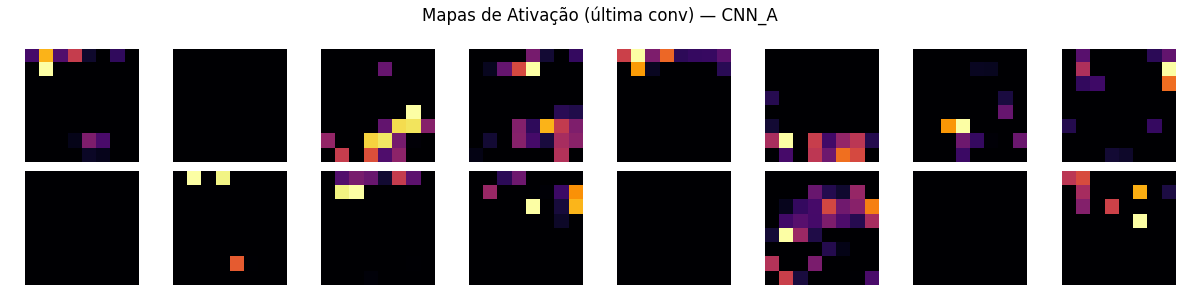
\includegraphics[width=0.7\textwidth]{output/CNN_A_mapas_ativacao.png}
    \caption{Mapas de ativação (última camada convolucional) da CNN-A.}
    \label{fig:cnn_a_mapas}
\end{figure}

\subsection{CNN-B}

\subsubsection{Acurácia, Loss e Predições}
A CNN-B apresentou o melhor desempenho da bateria de testes, alcançando uma acurácia de 83.00\%. O treinamento prosseguiu até a época 47, denotando um aprendizado prolongado e resiliente. O uso de uma janela perceptiva maior no início ($5 \times 5$) em conjunto com um \textit{dropout} leve de 10\% propiciou uma evolução suave. Observa-se na Figura \ref{fig:cnn_b_hist} que a distância (\textit{gap}) entre as curvas de validação e treino manteve-se estreita e sob controle na maior parte do processamento. A Figura \ref{fig:cnn_b_pred} exemplifica as saídas na fase de predição.

\begin{figure}[htpb]
    \centering
    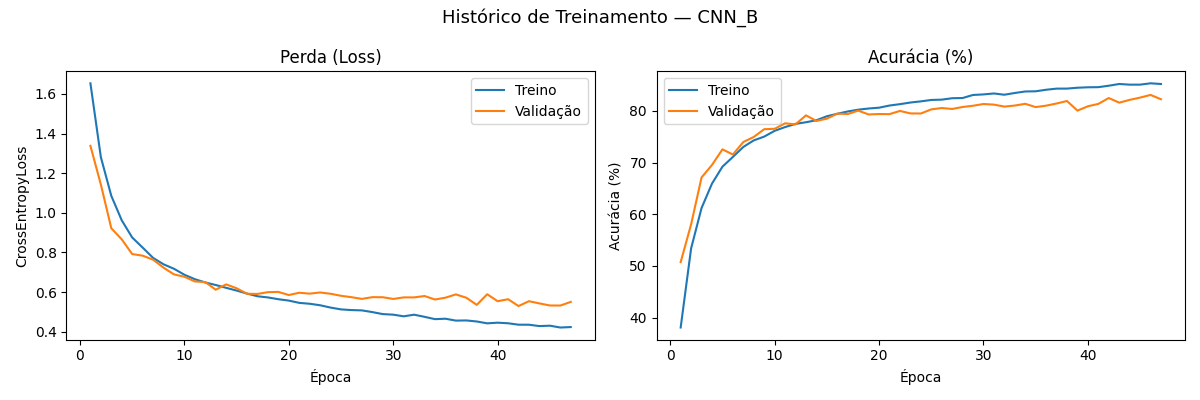
\includegraphics[width=0.9\textwidth]{output/CNN_B_historico.png}
    \caption{Histórico de \textit{Loss} e Acurácia para a CNN-B.}
    \label{fig:cnn_b_hist}
\end{figure}

\begin{figure}[htpb]
    \centering
    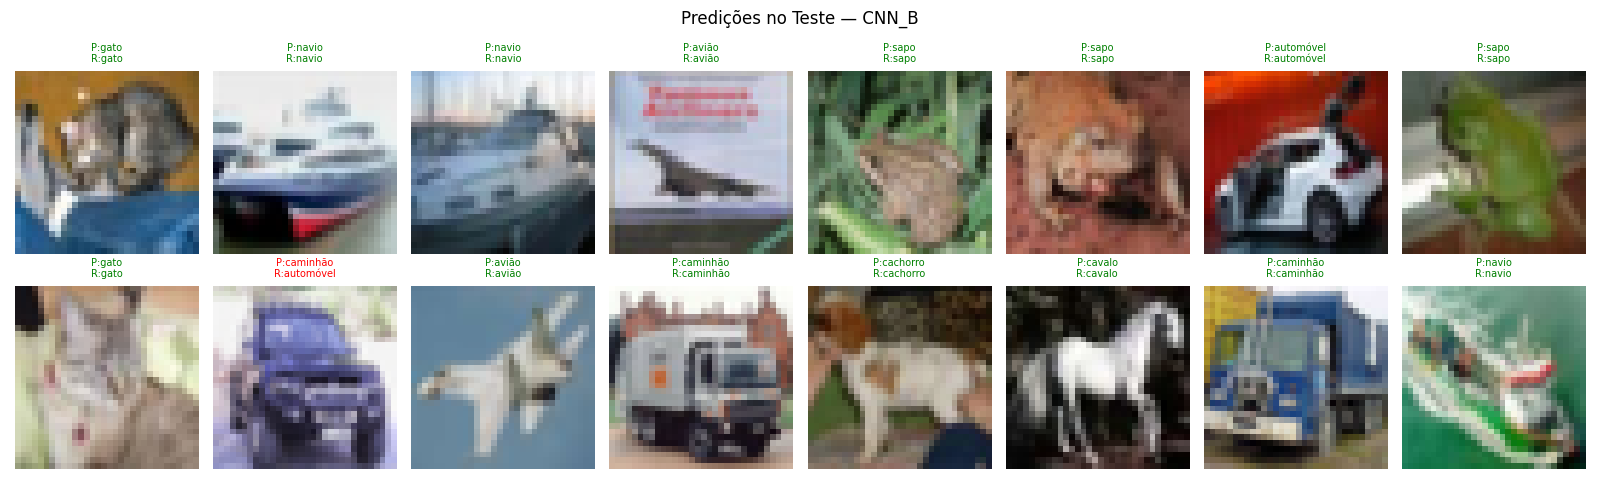
\includegraphics[width=0.8\textwidth]{output/CNN_B_predicoes.png}
    \caption{Amostra de predições da arquitetura CNN-B no conjunto de teste.}
    \label{fig:cnn_b_pred}
\end{figure}

\subsubsection{Filtros e \textit{Feature Maps}}
Os kernels maiores da camada inicial (Figura \ref{fig:cnn_b_filtros}) permitiram a captura englobante de texturas variadas e gradientes de fundo de forma mais expressiva que a arquitetura predecessora. Os \textit{feature maps} resultantes (Figura \ref{fig:cnn_b_mapas}) ilustram um isolamento notório das características de interesse (e.g., contornos de carros ou focinhos), reduzindo significativamente o nível de ruído propagado para a camada de predição linear.

\begin{figure}[htpb]
    \centering
    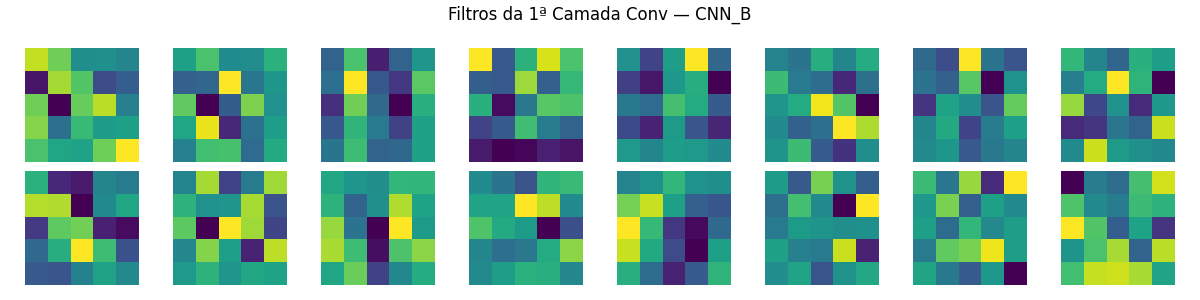
\includegraphics[width=0.7\textwidth]{output/CNN_B_filtros.png}
    \caption{Filtros aprendidos na primeira camada convolucional da CNN-B.}
    \label{fig:cnn_b_filtros}
\end{figure}

\begin{figure}[htpb]
    \centering
    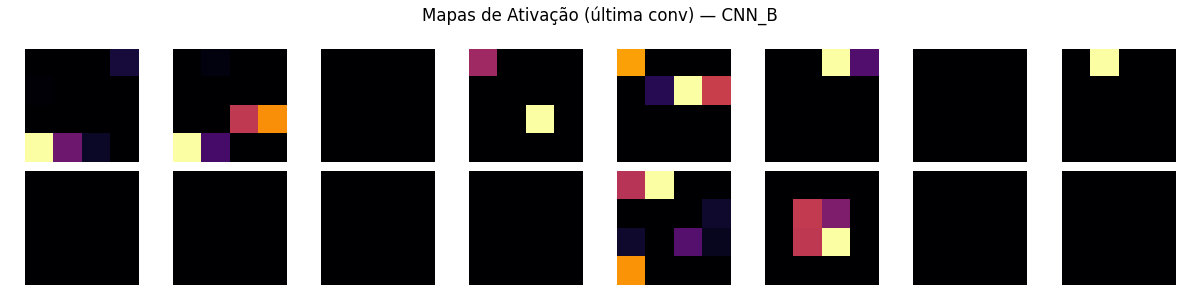
\includegraphics[width=0.7\textwidth]{output/CNN_B_mapas_ativacao.png}
    \caption{Mapas de ativação (última camada convolucional) da CNN-B.}
    \label{fig:cnn_b_mapas}
\end{figure}

\subsection{CNN-C}

\subsubsection{Acurácia, Loss e Predições}
Tratando-se do modelo mais profundo da análise (4 camadas convolucionais), a CNN-C finalizou a rotina com 82.23\% de acurácia de teste, parando o processo antecipadamente na época 34. A configuração aliada ao otimizador \textit{SGD} e uma forte taxa de \textit{dropout} (0.3) provocou um comportamento oscilatório acentuado ao longo das épocas (Figura \ref{fig:cnn_c_hist}). Todavia, a capacidade da rede de manter uma correlação íntima entre o conjunto de treinamento e de validação reforça sua alta tolerância contra a memorização (\textit{overfitting}).

\begin{figure}[htpb]
    \centering
    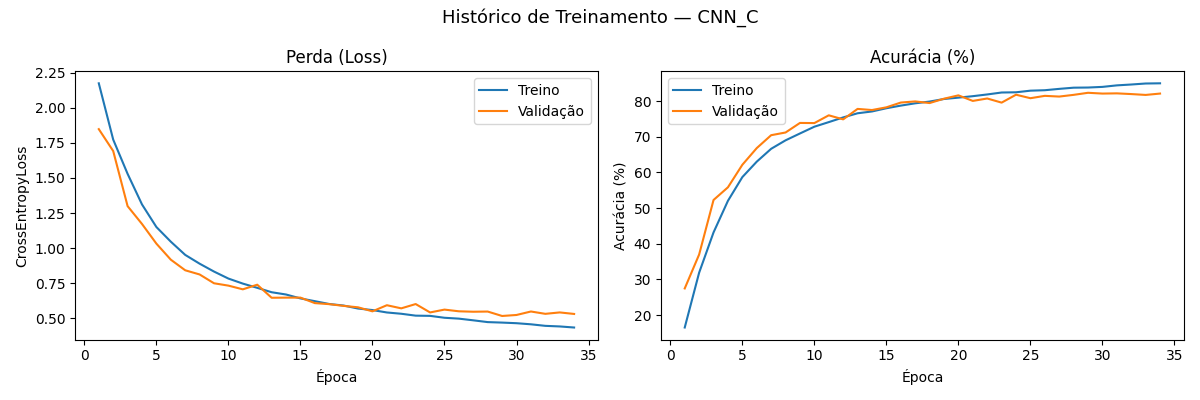
\includegraphics[width=0.9\textwidth]{output/CNN_C_historico.png}
    \caption{Histórico de \textit{Loss} e Acurácia para a CNN-C.}
    \label{fig:cnn_c_hist}
\end{figure}

\begin{figure}[htpb]
    \centering
    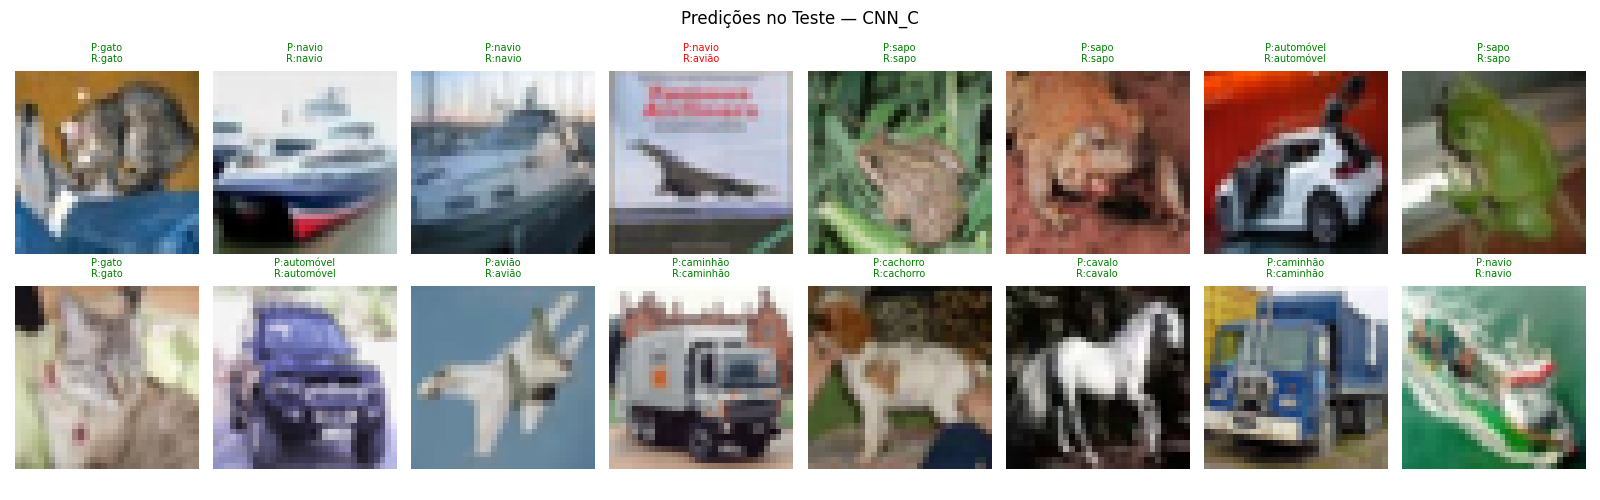
\includegraphics[width=0.8\textwidth]{output/CNN_C_predicoes.png}
    \caption{Amostra de predições da arquitetura CNN-C no conjunto de teste.}
    \label{fig:cnn_c_pred}
\end{figure}

\subsubsection{Filtros e \textit{Feature Maps}}
Na CNN-C, as visualizações dos filtros iniciais (Figura \ref{fig:cnn_c_filtros}) exibem aprendizado direcionado a frequências espaciais específicas e direcionais. Em decorrência das intensivas operações sub-consequentes de \textit{max-pooling}, os \textit{feature maps} profundos (Figura \ref{fig:cnn_c_mapas}) exibem blocos semânticos extremamente abstratos. Nesse ponto, o conceito visual tradicional dá lugar a mapeamentos pontuais (\textit{hotspots}) que a porção densa da rede utiliza para definir a qual classe os vetores latentes pertencem.

\begin{figure}[htpb]
    \centering
    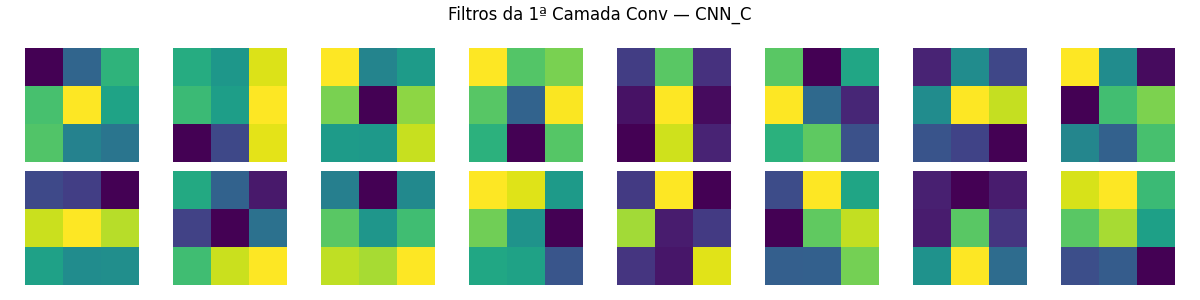
\includegraphics[width=0.7\textwidth]{output/CNN_C_filtros.png}
    \caption{Filtros aprendidos na primeira camada convolucional da CNN-C.}
    \label{fig:cnn_c_filtros}
\end{figure}

\begin{figure}[htpb]
    \centering
    
\includegraphics[width=0.7\textwidth]{output/CNN_C_mapas_ativacao.png}
    \caption{Mapas de ativação (última camada convolucional) da CNN-C.}
    \label{fig:cnn_c_mapas}
\end{figure}

% ===========================================================================
\section{Conclusão}
% ===========================================================================

O presente estudo avaliou a performance de três topologias de Redes Neurais Convolucionais empregadas na classificação do agrupamento \textit{CIFAR-10}. A Figura \ref{fig:comparacao} condensa a performance objetiva obtida em \textit{holdout} (teste), indicando a superioridade da configuração da CNN-B (83.00\%).

\begin{figure}[htpb]
    \centering
    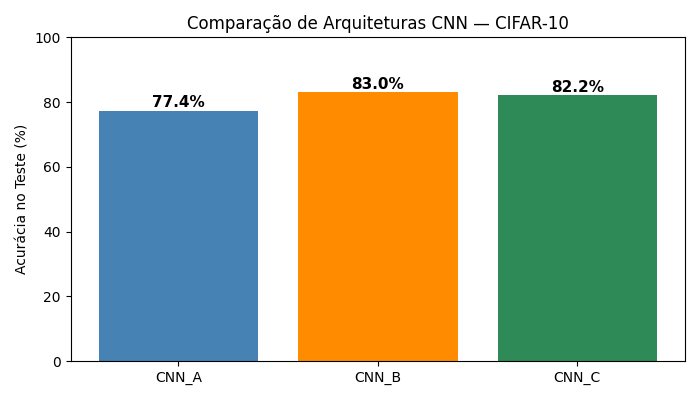
\includegraphics[width=0.6\textwidth]{output/comparacao_arquiteturas.png}
    \caption{Comparação final da acurácia de teste entre as três arquiteturas avaliadas.}
    \label{fig:comparacao}
\end{figure}

Conclui-se que o ganho escalar na capacidade de abstração espacial não depende puramente de redes extensamente rasas (CNN-A), que tendem a saturar rapidamente
. Em vias simétricas, arquiteturas sensivelmente mais profundas (CNN-C) necessitam de sintonia fina prolongada, como demonstrado pelas flutuações relativas ao otimizador SGD
. A configuração CNN-B se consagra empíricamente como o ponto de equilíbrio ideal no contexto destas dimensões de imagem ($32 \times 32$); operando com filtros estendidos na captação inicial e uma regularização contida de \textit{dropout}, sem desestabilizar os pesos com o passar das épocas. Por fim, valida-se o impacto crítico do pipeline de \textit{Data Augmentation}, sendo vital como mecanismo contínuo de imunização das redes contra o fenômeno perene do sobreajuste.


\end{document}

\end{document}
